\documentclass[a4paper]{article}

\usepackage{amsmath}
\usepackage{enumitem}

\usepackage{caption}
\usepackage{subcaption}

\usepackage{graphicx}
\author{Kennard Ng and Luo Wen Han}
\title{Project 1: Manhattan World}

\bibliographystyle{unsrt}

\begin{document}
	\maketitle
	\section{Introduction}
	
	In this project, we use the expectation maximization framework to simultaneously obtain the extrinsic camera parameters i.e. the camera's rotation matrix and its translation, and the vanishing points of the image. 
	
	This problem is a chicken-and-egg problem where the extrinsic camera parameters are needed to determine the vanishing points, and the vanishing points can be used to deterimine the extrinsic camera parameters. 
	
	We apply the expectation maximization framework to images that are consistent with the Manhattan World Assumption, where 
	%todo: manhattan world assumption her. 
	
	\section{Background}
	
	\subsection{Perspective Projection}
	
	Perspective transformations are extensively used in Computer Vision because they model the transformation of 3D points 
	
	\subsection{Vanishing Points}
	
	Under perspective projection, parallel lines in the 3D world appears to converge in images e.g. Figure \ref{fig:vp_eg}.
	
	\begin{figure}[ht]
		\centering
		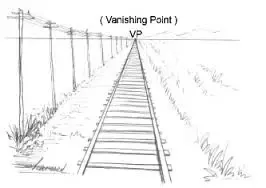
\includegraphics[width=0.5\linewidth]{images/vp_eg}
		\caption{Vanishing Point Example}
		\label{fig:vp_eg}
	\end{figure}

	The point of convergence is known as the vanishing point with lines in the image pointing towards the vanishing point being described as vanishing lines. Pixels that lie on vanishing lines tend to have the same image gradient given that lie on the same line. 
	
	\section{Our Approach}
	
	In our approach, we define the rotation matrix by its euler angles: $\alpha$, $\beta$ and $\gamma$. $\alpha, \beta$ and $\gamma$ are the rotation angles about the $x, y$ and $z$ axes respectively. 
	
	
	
	\subsection{Initialization}
	
	We use the coarse-to-fine search strategy proposed in~\cite{Coughlan:2000:MWA:3008751.3008869} to intialize euler angles before performing expectation minimization. In this search strategy, we explore discrete values to obtain a rough estimate of the camera parameters. From the search, we select the values that maximize the posterior over the search range:
	
	\begin{equation}
		P\left(M | G, \Psi\right) \propto P\left(G | M, \Psi\right) P(M),
	\end{equation}
	
	where $M, G$ and $\Psi$ denotes the assignment of pixels to vanishing points, the gradients of the pixels, and the euler angles respectively. The likelihood $P\left(G | M, \Psi \right)$ is given by: 
	\begin{equation}
	P\left(G | M, \Psi \right)=\left\{\begin{array}{ll}\mathcal{N}(0, 0.5) & {\text { if } m = \{1, 2, 3\}} \\ {1 / 2\pi} & {\text { if } m=4}\end{array}\right.
	\end{equation}
	
	where $m=\{1,2,3\}$ denotes the assignment to vanishing points from the natural cartesian grid of the image and $m={4}$ denotes an assignment to other vanishing points present in the image. Given that we wish to maximize the posterior across all pixels $p$, we find euler angles that maximize the following:
	\begin{equation}
		\Psi^*=\operatorname{argmax}_\Psi \prod_p P(G_p|M,\Psi)P(M) = \operatorname{argmax}_{\Psi} \prod_{p} \sum_{m=1}^4 P\left(G_p|m, \Psi\right)p(m)
	\end{equation}
	
	Computing $\Psi^*$ using the above approach is computationally intractable since $\prod_p P(G_p|M,\Psi)P(M) \rightarrow 0$ as $p$ increases. Hence, we use the log trick to make it tractable and compute $\Psi^*$ as follows:
	
	The coarse-to-fine search begins with a coarse search for $\beta$ over the range $-\pi / 3$ to $\pi / 3$ at increments of $\pi / 90$, with $\alpha, \gamma = 0$. The result of the coarse seach if the optimal coarse search value $\beta_c$.
	
	Then, a fine search is performed over $\alpha, \beta_c, \gamma$. Specifically, we explore over small permutations of $\pi / 90$ from $\beta_c$ for $\beta$,  $\pi / 36$ from $0$ for $\alpha$ and $\gamma$.
	
	
	\section{Vertibi Algorithm}
	
	We use the Vertibi Algorithm in our formulation. The Vertibi algorithm is based on dynamic programming and at each vertibi $v_i$, it computes the vertibi which is the minimum configuration given the previous $i-1$ hidden states and the $i$ observations. It uses the following recursive formulation:
	
	\begin{equation}
		v_i = \min_{0\cdots c-1} v_{i-1}\text{Pr}_{em}\text{Pr}_{tr},
		\label{eqn:vertibi}
	\end{equation}
	where $\text{Pr}_{em}$ and $\text{Pr}_{tr}$ represents the emission probability of a pixel in the current row and the transition probability from the pixel in the higher row (in the previous iteration) that gives the minimum configuration for $v_{i-1}$ into the pixel in the present row, respectively. We formulate \ref{eqn:vertibi} in a log-linear form as well:
	\begin{equation}
		v_i = \min_{0\cdots c-1} v_{i-1} + \log\text{Pr}_{em} + \log\text{Pr}_{tr},
	\end{equation}	
	and each seam has a final vertibi $v_{r-1}$, where a seam begins from a pixel along the top row of the image. At each iteration, we have $c_t$ seams, where $c_t$ is the number of columns of the image at iteration $t$. We select the seam with the minimum vertibi $v_{r_{t-1}}$  at each iteration and remove it, by shifting the pixels on the right of the seam to the left by one pixel. 
	
	The pseudo code of our implementation of the Seam Carving algorithm is given below: \\
	
	\textbf{Seam Carving Algorithm}
	\begin{enumerate}[noitemsep]
		\item Repeat for $T$ iterations until desired image size:
		\begin{enumerate}[noitemsep]
			\item Let the iteration be $t$, number of rows of the image be $r$, and the number of columns be $c_t$.
			\item Run Vertibi algorithm and backtrack from the algorithm to get the location of the pixels that form the seam with the minimum vertibi.
			\item Remove the seam pixels by shifting the pixels on the right of the seam to the left.
		\end{enumerate}
	\end{enumerate} 
	
	\textbf{Vertibi Algorithm}
	\begin{enumerate}[noitemsep]
		\item Let the $v_\text{min} = \infty$
		\item For $j = 0, \cdots, c_t-1$, 
		\begin{enumerate}[noitemsep]
			\item Let the starting pixel be the pixel indexed by $0,k$, where $k=j$ initially.
			\item Let $v_0 = x_{0,j}$.
			\item For $i=1, \cdots, r-1$, compute $v_i = v_{i-1}\min_k x_{i,k}$ for $k \in \left\{j-1, 0, j+1\right\}$. 
			\item Update $v_\text{min} = \min(v_{r-1}, v_\text{min})$ 
		\end{enumerate}
		\item Backtrack $v_\text{min}$ and return the pixel locations of the seam with the minimum configuration.
	\end{enumerate}
	
	\section{Qualitative Results}
	
	These are our qualitative results:
	
	From our results, we see that important parts of the image i.e. the person and the castle have been preserved during the resize operation, where their scale have been preserved. On the other hand, unimportant parts of the iamge i.e. background has been carved away during the resize operation.
	

	
	\bibliography{references.bib}
	
\end{document}